%!TEX encoding = UTF-8 

% ugly and possibly dangerous command
%\setcounter{page}{15}

\chapter{Introduction}

%%%%%%%%%%%
\section{Motivation}

A current field of research in humanoid robotics\index{humanoid robotics} is the study of \emph{interactions} between a robot and its human users, focusing on topics such as perception\index{perception}, learning and imitation. Neurosciences\index{neurosciences} and developmental psychology\index{developmental psychology|see{psychology}}\index{psychology}, which study the inner mechanisms of the human brain, also contribute to these matters as they try to understand key cognitive\index{cognition} issues: how to learn sensory-motor coordination\index{sensory-motor coordination}, which properties of observed objects or of the world we learn, how human beings imitate\index{imitation} each other, and how they recognize actions.

The reason why interactions are relevant and worth studying in robotics is twofold. First, they allow us to progress within the underlying scientific disciplines: robotics, image processing, \ac{CV}, \ac{AI}, signal processing and control theory.

Secondly, by improving human-robot interactions\index{interactions} and better understanding our brain\index{cognition}, we also contribute to specific applications that have an increasing \emph{social impact}, namely rescue operations, emergencies, visual monitoring of urban areas, as well as robotic assistants that improve quality of life for the elderly or disabled people~\cite{hu:2007}.

\begin{figure}
\centering
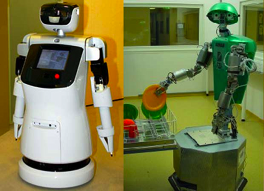
\includegraphics{figures/service_robots}
\caption[Example of service robots]{Two examples of service robots, built by the University of Karlsruhe (Germany) and Fujitsu, respectively.}
\label{img:service_robots}
\end{figure}

Grasping\index{grasping} and manipulation\index{manipulation} are among the most fundamental tasks to be considered in humanoid robotics\index{humanoid robotics}. Fig.~\ref{img:service_robots} shows two examples of service robotics platforms that possess enough tools, appliances and flexibility to potentially adapt to human tasks\index{imitation}.

Just like humans distinguish themselves from other animals by having highly skilled hands, so can humanoid robots: dexterous ability must be considered as a key component in practical applications such as service robotics or personal robot assistants.

The high dexterity that characterizes human manipulation does not come for granted at birth. Instead, it arises gradually during a complex developmental process which spans different stages. After recognizing things surrounding them by the means of \emph{vision}, babies first attempt to reach for these things, with a very limited precision. Then, at some point they start to adapt their hands to the shape of objects, initially letting these objects fall on the ground because of incorrect grasping procedures. Only after some years are they finally able to master their arm and hand skills.

Furthermore, perception\index{perception} develops in parallel with these manipulation\index{manipulation} skills, in order to incrementally increase the performance in detecting and measuring those object features that are important for touching, grasping\index{grasping} and holding something. Along time, interactions with objects of diverse shapes are successfully performed by applying various possible reaching\index{reaching} and manipulation techniques. Salient\index{saliency} effects are produced (e.g., an object moves, it is deformed, or it makes a sound when squeezed), perceived and associated to actions. An agent thus learns object affordances~\cite{montesano:2008}\index{object affordances}\index{affordances|see{object affordances}}, i.e., the relationships among a certain manipulation\index{manipulation} action, the physical characteristics of the object involved, and the observed effects. The way of reaching for an object evolves from a purely position-based mechanism to a complex behaviour which depends on target size, shape, orientation\index{orientation}, intended usage and desired effect.

Framed within the \ac{RobotCub} Project~\cite{metta:2005}\index{RobotCub}, this thesis aims at providing \emph{simple} 3D object perception\index{perception} for enabling the development of manipulation\index{manipulation} skills in a humanoid robot\index{humanoid robotics}, by approximating a perceived object with its best-fit enclosing ellipse\index{ellipse}. 

This work addresses the problem of reaching\index{reaching} for an object and preparing the grasping\index{grasping} action, according to the \emph{orientation}\index{orientation} of the objects to interact with. The proposed technique is not intended to have very accurate measurements of object and hand postures, but merely the necessary quality to allow for successful object--hand interactions. Precise manipulation\index{manipulation} needs to emerge from experience by optimizing action parameters as a function of the observed effects. To have a simple enough model of object and hand shapes, they are approximated as 2D ellipses\index{ellipse} located in a 3D space. An underlying assumption is that objects have a sufficiently \emph{distinct colour}, in order to facilitate segmentation\index{image segmentation} from the image background. Perception\index{perception} of object orientation\index{orientation} in 3D is provided by the second-order moments of the segmented areas in left and right images, acquired by a humanoid robot active vision head.

This thesis will describe: the humanoid robot platform ``Baltazar'' that was used for research and tests, the adopted \ac{CV} techniques, a simple method to estimate the 3D orientation of a target object, strategies for the reaching and grasping tasks, experimental results and future work.

%%%%%%%%%%%%%%%%%%%%%%%%%%%%%%%%%%%%%%%
\section[RobotCub]{RobotCub and the Development of a Cognitive Humanoid Robot}
\index{RobotCub}

\begin{figure}
\centering
\subfloat[][RobotCub Consortium logo.]
{
\includegraphics[width=.55\columnwidth]{figures/robotcub} \label{img:robotcub} } \quad
% %necessary to prevent line break
\subfloat[][The iCub robot platform standing.]
{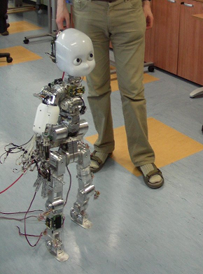
\includegraphics[width=.35\columnwidth]{figures/icub_standing} \label{img:icub_standing} }
\caption[RobotCub logo and iCub baby robot prototype]{RobotCub logo and a prototype of its baby robot prototype, the iCub.}
\label{fig:robotcub-icub}
\end{figure}

The \ac{RobotCub} Consortium~\cite{link:robotcub}\index{RobotCub} is a five-year-long project, funded by the European Commission through Unit E5 (``Cognition'') of the Information Society Technologies priority of the Sixth Framework Programme (FP6). 

\ac{RobotCub} is a project to study cognition through robotics. Its objective is to create a completely open design for a humanoid robot --- ``open hardware,
open software, open mind''. All the \ac{RobotCub} hardware designs and software are free and open source\index{open source}. The \ac{RobotCub} Consortium is composed of 16 partners: 11 from Europe, 3 from Japan and 2 from the USA. LIRA-Lab~\cite{link:liralab} at the University of Genoa, Italy, is the coordinator.

Inspired by recent results in neurosciences\index{neurosciences} and developmental~psychology\index{psychology}, the objective of \ac{RobotCub} is to build an open-source humanoid platform for original research on cognitive robotics, with a focus on developmental aspects. One of the tenets of the project is that manipulation\index{manipulation} plays a key role in the development of cognitive ability.

% balta_workspace is not used atm

%\begin{figure}
%\centering
%\subfloat[][The iCub robot platform standing.]
%{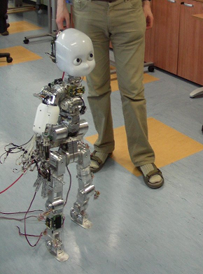
\includegraphics[width=.35\columnwidth]{figures/icub_standing} \label{img:icub_standing} } \quad
% %necessary to prevent line break
%\subfloat[][Baltazar robot platform in its workspace.]
%{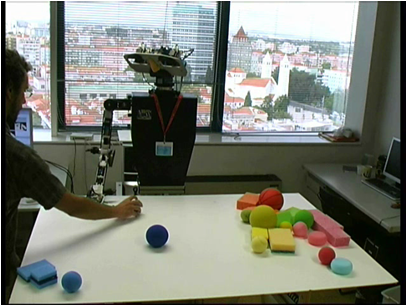
\includegraphics[width=.55\columnwidth]{figures/balta_workspace} \label{img:balta_workspace} }
%\end{figure}

The iCub\index{iCub}\label{icub} is a humanoid baby robot designed by the \ac{RobotCub} consortium. The iCub, shown in Fig.~\ref{img:icub_standing}, is a full humanoid robot the size of a two-year-old child. Its total height is around 90 cm, and it has 53 \acp{DOF}, including articulated hands to be used for manipulation\index{manipulation} and gesturing; in addition, the iCub is equipped with an inertial system in its hand, stereo audition, and the ability to perform facial expressions.

At the time of writing this thesis, a study is being conducted for determining if and how many \acp{DOF} are minimally required to produce and generate plausible facial expressions. The iCub\index{iCub} robot should eventually be able to crawl and sit (to free the hands from supporting the body) and autonomously transition from crawling to sitting and vice-versa. 

This thesis work was carried out at the Computer and Robot Vision Laboratory~\cite{link:vislab}, Institute for Systems and Robotics, IST, Lisbon (Portugal) during 2008. At the time of working on this project, the arm-hand system of a full iCub prototype was still being assembled. Therefore, for this work another humanoid robot platform was used: Baltazar~\cite{lopes:2004, lopes:2007}\index{Baltazar}. It consists of a robotic torso and a binocular head, built with the aim of understanding and performing human-like gestures, mainly for biologically inspired research.

%%%%%%%%%%%%%%%
\section{Thesis Background}

Manipulation skills\index{manipulation} at macro- and micro-scales are very important requirements for robot applications. This is valid both in industrial robotics\index{industrial robotics} and in less-traditional fields. As far as industry is concerned, robot manipulators hold a key role in many scenarios; to name a few:
\begin{itemize}
\item handling;

\item food;

\item fabrics;

\item leather.
\end{itemize}

Similarly, in less structured domains of robotics, manipulation still play a relevant part:
\begin{itemize}
\item surgery;

\item space;

\item undersea.
\end{itemize}

Manipulation and grasping systems are thus a vital part of industrial, service and personal robotics, they are employed in various applications and environments, not just in advanced manufacturing automation as one may intuitively think.

\begin{figure}
\centering
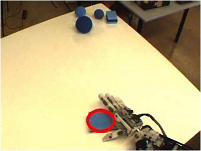
\includegraphics{figures/balta_grasping}
\caption[Baltazar humanoid robot and its workspace]{Humanoid robot Baltazar operating in its workspace, as seen from one of its cameras. The anthropomorphic hand of Baltazar is reaching for a visually-tracked object and is about to grasp it.}
\label{img:balta_grasping}
\end{figure}

Actuating a robotic limb is not merely commanding it to a given position: the issue is also where and how to move it, and for this purpose \ac{CV} (the ability for machines to understand images) is a powerful tool that can assist humanoid robotics broadly. In particular, \ac{CV} is used for robot manipulation tasks: reaching for something, touching or grasping it.

A major difficulty for humanoid robots in order to successfully perform a grasping task is the \emph{variety of objects} they have to interact with: a robot should be able to see and understand any shape and size, including never-before-seen objects. To do this, deploying simple \emph{model-free} methods (i.e., not enforcing any model) is often the sensible choice to follow, including in the approach presented in this thesis.

In particular, our objective is to approximate an object positioned in front of a humanoid robot with its smallest \emph{enclosing ellipse}\index{ellipse}. In addition, the target object may not necessarily be static, so the developed techniques must also cope with following where this target is moving. This is done by the means of \ac{CAMSHIFT} trackers.

A computer vision technique to estimate the 3D position and orientation of a moving target object placed in front of a humanoid robot, equipped with a stereo rig, will be presented. The information inferred will subsequently be used by the robot to better \emph{interact} with the object, that is, to manipulate it with its arm: an approach for real-time preparation of grasping tasks is described, based on the low-order moments of the target's shape on a stereo pair of images acquired by an active vision head.

\label{intro:reaching_phases}
To reach for an object\index{reaching}, two distinct phases are considered~\cite{lopes:2007}:
\begin{enumerate}
\item an open-loop ballistic phase to bring the manipulator to the vicinity of the target, whenever the robot hand is not visible in the robot's cameras;

\item a closed-loop visually controlled phase to accomplish the final alignment to the grasping position.
\end{enumerate}

The open-loop phase (reaching preparation) requires the knowledge of the robot's inverse kinematics and a 3D reconstruction of the target's posture. The target position is acquired by the camera system, where the hand position is measured by the robot arm joint encoders. Because these positions are measured by different sensory systems, the open-loop phase is subject to mechanical calibration errors. The second phase (grasping preparation), operates when the robot hand is in the visible workspace. 3D position and orientation of target and hand are estimated in a form suitable for \acl{PBVS} (\acs{PBVS})~\cite{chaumette:visual1, hutchinson:1996}. The goal is to make the hand align its posture with respect to the object. Since both target and hand postures are estimated in the same reference frame, this methodology is not prone to significant mechanical calibration errors.

%%%%%%%%%%%%%%%%
\section{Problem Statement}

The objective is to estimate the 3D position and orientation of an object placed in front of a humanoid robot, in order for make it possible to interact and manipulate such object. This estimation is done in two visual processing steps: tracking the object shape as it (possibly) moves within the robot stereo cameras' 2D vision, then combining the inferred information through 3D reconstruction methods.

Computation must be real-time, so that the understanding of a dynamic scene and the interactions with objects are accurate but also usable in practical experiments. This constraint calls for a simplified, model-free vision approach. An object position and orientation will be approximated with its best-fit enclosing ellipse.

Furthermore, the employed software components must be clearly decoupled, in order to make it possible to adapt them to other robotic platforms and scenarios (such as a full iCub robot; see p.~\pageref{icub}).

Finally, the geometric measurements acquired so far should to be used for the two phases of a reaching task, necessary for object manipulation: (i) an initial phase whereby the robot positions its hand close to the target with an appropriate hand orientation, and (ii) a final phase where a precise hand-to-target positioning is performed using Visual~Servoing methods.

%%%%%%%%%%%%%%
\section{Thesis Structure}

The thesis is organized as follows:

%
\begin{itemize}
\item Chapter~\ref{chap:related_work} lists the existing techniques for segmentation, stereo~vision (in particular 3D reconstruction) and manipulation tasks for humanoid robots;

\item Chapter~\ref{chap:robot_platform} describes the structure of the robot used in our development and experiments, ``Baltazar'', as well as the software libraries and tools that make up this work;

\item Chapter~\ref{chap:proposed_architecture} details the \ac{CAMSHIFT} tracker implementation, the 3D reconstruction software module and the proposed manipulation approach;

\item Chapter~\ref{chap:experimental_results} displays the behaviour and results obtained with the developed work;

\item Chapter~\ref{chap:conclusions} draws the concluding remarks and it outlines some possible ways to continue the research work started in this thesis.
\end{itemize}